\documentclass[a4paper,12pt,oneside,onecolumn,final]{EEIMVR}
% ---
% Pacotes fundamentais 
% ---

\usepackage{lipsum}
% ---
% Pacote auxiliar para as normas da UFF
% ---
\usepackage[frame=no,font=sans]{EEIMVRformat} %font=sans (arial), font=times, font=default ou font=lmodern

% --- Pacotes adicionais usados neste trabalho ---
\usepackage{float}
\usepackage{tikz}
\usetikzlibrary{positioning,calc,arrows.meta}
\usepackage{pgfplots}
\pgfplotsset{compat=1.18}
\usepackage[portuguese]{algorithm2e}
\usepackage{listings}
\definecolor{commentgray}{gray}{0.4}
\lstset{
  language=C,
  basicstyle=\ttfamily\small,
  keywordstyle=\bfseries,
  commentstyle=\itshape\color{commentgray},
  numbers=none, frame=single, framerule=0.4pt,
  breaklines=true, showstringspaces=false, captionpos=b,
  xleftmargin=1em, aboveskip=1.2em, belowskip=1em,
  literate=%
    {á}{{\'a}}1 {à}{{\`a}}1 {â}{{\^a}}1 {ã}{{\~a}}1
    {é}{{\'e}}1 {ê}{{\^e}}1 {í}{{\'i}}1
    {ó}{{\'o}}1 {ô}{{\^o}}1 {õ}{{\~o}}1
    {ú}{{\'u}}1 {ç}{{\c c}}1
    {Á}{{\'A}}1 {É}{{\'E}}1
}
\renewcommand{\lstlistingname}{Listagem}
\renewcommand{\lstlistlistingname}{Lista de listagens}

% ---
% Pacote de citacoes
% ---
\usepackage[alf, abnt-repeated-author-omit=no, abnt-emphasize = bf, abnt-full-initials=no, abnt-thesis-year=final]{abntex2cite}

% **********************************************************
% **********************************************************
% Informações de autoria e institucionais
% **********************************************************
% **********************************************************

%-----------------------------------------------------------
% Grau pretendido (Doutor, Mestre, Bacharel, Licenciado) e Curso
%-----------------------------------------------------------


\grau{Graduação}
% \grau{Mestre} 
%\grau{Doutor}


\curso{Física Computacional}


\areadeconcentracao{} %Projeto de Graduação
% \areadeconcentracao{Fenômenos de Transporte} %Pós Graduação
%\areadeconcentracao{Mecânica dos Sólidos} %Pós Graduação

%-----------------------------------------------------------
% Informações da instituição
%-----------------------------------------------------------
\instituicao{Universidade Federal Fluminense}  %Universidade
            {} % Polo Universitário
            {Instituto de Ciências Exatas} %Unidade
            { Curso de Bacharelado em Física  Computacional}

%-----------------------------------------------------------
% Informações da autoria do documento
%-----------------------------------------------------------

\autor{Vinícius Santos Anjos da}
      {Silva}
      {} % iniciais do nome (opcional)

\titulo{Modelagem baseada em agentes paralelizada em CUDA: o impacto da COVID-19 em áreas urbanas no Brasil}

\orientador{Prof. Dr.} %cargo
		   {Aquino Lauri} %nome
           {de Espíndola} %sobrenome
           {UFF -- Universidade Federal Fluminense -- VVR} % Instituição

%Opcional, Comente as linhas de coorientador caso não tenha
%\coorientador{Prof. Dr.}{Nome}{Sobrenome}{unidade -- instituição}

%-----------------------------------------------------------
% Informações adicionais (local, data e paginas)
%-----------------------------------------------------------

\local{Volta Redonda, RJ}
\data{XX}{mês}{2026} % preencher com a data da defesa

% ***********************************************************
% ***********************************************************
% Início do documento
% ***********************************************************
% ***********************************************************

\begin{document}
% ----------------------------------------------------------
%% ELEMENTOS PRE-TEXTUAIS
% ----------------------------------------------------------
\frontmatter
% ----------------------------------------------------------ENGENHARIA
% Capa e a folha de rosto
% ----------------------------------------------------------
\capa % use \capa* para ir para o seguundo modelo de capa
\folhaderosto
% ----------------------------------------------------------
% Inserir a ficha catalográfica
% ----------------------------------------------------------
% ---
% A biblioteca deverá providenciar a ficha catalográfica. Salve a ficha no
% formato PDF. Use o nome do arquivo PDF como argumento do comando. 
% Exemplo: ficha catalográfica é o arquivo 'Ficha.pdf' na pasta "B.PreTextual"
%     \fichacatalografica{B.PreTextual/Ficha.pdf}
%
% Enquanto não possuir a ficha catalográfica, use o comando sem argumentos.
% ---
% \includepdf[noautoscale, pagecommand={}]{B.PreTextual/Ficha.pdf} % Substituir o arquivo ficha.pdf pela sua ficha catalográfica

\vspace*{9cm}

\noindent
\textbf{A Ficha Catalográfica é elaborada pela Biblioteca do Aterrado - BAVR}

\bigskip
\noindent
Endereço para solicitar a ficha catalográfica: \url{https://bibliotecas.uff.br/bavr/}

\bigskip
\noindent
O link acima informa os itens necessários para solicitação da ficha.

\bigskip
\noindent
A ficha catalográfica deve ser inserida na parte inferior da folha. Para inserção da ficha, é recomendado o uso de caixa de texto.

\vspace{2.5cm}

\noindent\fbox{\begin{minipage}[t][8cm][t]{\dimexpr\textwidth-2\fboxsep-2\fboxrule\relax}
ESPAÇO PARA INSERIR A FICHA CATALOGRÁFICA
\end{minipage}}
% After this page is finished, remove the includepdf command of main.tex




% ----------------------------------------------------------
% Folha de aprovação
% ----------------------------------------------------------

%Após obter a assinatura dos membros da banca, comente as linhas a baixos e insira o pdf com as assinaturas na pasta "B.PreTextual"


% Ajustar o espaço entre as assinaturas abaixo
\newcommand{\spc}{0.25cm}

\begin{folhadeaprovacao}
	\vspace{\spc} % Espaço entre assinaturas
	\assinatura{Prof(a). Dr(a). Nome }{instituição } %Exemplo
 	\vspace{\spc} % Espaço entre assinaturas
\assinatura{Prof(a). Dr(a). Nome }{instituição } %Exemplo
% 	\vspace{\spc} % Espaço entre assinaturas
% 	\assinatura{Eng. Marcos João, B.Sc.}{Instituição}
% 	\vspace{\spc} % Espaço entre assinaturas
% 	\assinatura{quarto membro titular da banca}{Instituição}
\end{folhadeaprovacao}


% Após colocar o pdf com as assinaturas na pasta "B.PreTextual", comente todo o ambiente "folhadeaprovacao" acima, descomente a linha abaixo e insira o nome correto do arquivo pdf:
%\includepdf[pages=1]{B.PreTextual/ficha.pdf} %exemplo


% ----------------------------------------------------------
% Dedicatória
\pretextualchapter{Dedicatória}
\vfill
Eu dedico esse TCC para uma pessoa digna.






% ----------------------------------------------------------
% Agradecimentos
\pretextualchapter{Agradecimentos}

Agradeço a minha família, amigos e professores...



% ----------------------------------------------------------
% Epigrafe (opcional)
\pretextualchapter{}
\vfill
\begin{flushright}
	O homem é mortal por seus temores e imortal por seus desejos.\\
	\textit{Pitágoras}
\end{flushright}


% ----------------------------------------------------------
%% RESUMO
% se não for usar a quarta palavra chave, deixar o campo vazio: {}
\palavraschaves{Covid-19}
{Modelagem baseada em agentes}
{Programação paralela em GPU}
{CUDA}



\pretextualchapter{Resumo}

\noindent
As simulações epidemiológicas baseadas em agentes permitem representar a evolução de uma doença em uma população levando em conta as características individuais e espaciais dos indivíduos, porém, para áreas com grande número de indivíduos e diversos parâmetros, demandam elevado poder computacional. Este trabalho apresenta a paralelização, utilizando CUDA, de um modelo baseado em agentes do tipo SEIR estendido para a Covid-19, aplicado a quatro áreas urbanas brasileiras: São Paulo, Rocinha, Brasília e Manaus. A implementação em GPU é validada contra a implementação serial de referência sob os mesmos parâmetros, e o seu desempenho é avaliado por meio da aceleração e da eficiência. Os resultados mostram que a implementação paralela reproduz as curvas epidêmicas da implementação serial, com erro quadrático médio inferior a 1,2 ponto percentual, valor compatível com a flutuação estatística do método de Monte Carlo, e que a aceleração obtida cresce com o tamanho da rede, atingindo cerca de 56 vezes para a maior cidade. A análise de desempenho indica que a simulação é limitada pela largura de banda de memória, e uma otimização da estrutura de dados que mantém os acessos na memória cache reduz significativamente o tempo de execução.

\imprimirchaves % linha em branco antes


% ----------------------------------------------------------
% Abstract
\begin{otherlanguage}{english}
\keywords{Covid-19}
{Agent-based modeling}
{Parallel programming on GPU}
{CUDA}


\pretextualchapter{Abstract}

% O resumo em inglês deve ser organizado em apenas um parágrafo mesmo.
\noindent
Agent-based epidemiological simulations make it possible to represent the evolution of a disease in a population while accounting for the individual and spatial characteristics of the individuals; however, for areas with a large number of individuals and several parameters, they demand high computational power. This work presents the parallelization, using CUDA, of an extended SEIR agent-based model for Covid-19, applied to four Brazilian urban areas: São Paulo, Rocinha, Brasília and Manaus. The GPU implementation is validated against the reference serial implementation under the same parameters, and its performance is assessed through speedup and efficiency. The results show that the parallel implementation reproduces the epidemic curves of the serial implementation, with a root mean square error below 1.2 percentage points, a value compatible with the statistical fluctuation of the Monte Carlo method, and that the speedup grows with the lattice size, reaching about 56 times for the largest city. The performance analysis indicates that the simulation is limited by memory bandwidth, and a data-structure optimization that keeps memory accesses in the cache significantly reduces the execution time.

\printkeys % linha em branco antes

\end{otherlanguage}



% ----------------------------------------------------------
% Listas de ilustrações e tabelas
% ----------------------------------------------------------
\listoffigures % list of figures
\listoftables % list of tables
% ----------------------------------------------------------
% Outras listas
% ----------------------------------------------------------
%\listadealgoritmos


% ----------------------------------------------------------
% Lista de abreviaturas e siglas
\pretextualchapter{Lista de abreviaturas e siglas}
% ---
\addabbreviation{CITT}{Técnica da Transformada integral Clássica}
\addabbreviation{GITT}{Técnica da Transformada integral Generalizada}
\addabbreviation{MVF}{Método de Volumes Finitos}









% ----------------------------------------------------------
% Lista de simbolos
\pretextualchapter{Lista de símbolos}
% ---
\addsymbol{t}{Tempo}
\addsymbol{L}{Dimensão na direção $x$}
\addsymbol{H}{Dimensão na direção $y$}
\addsymbol{\rho}{Massa específica}
\addsymbol{\mu}{Viscosidade dinâmica}
\addsymbol{\nu}{Viscosidade cinemática}









% ----------------------------------------------------------
% Sumario
\tableofcontents % table of contents

% ----------------------------------------------------------
%% ELEMENTOS TEXTUAIS
% ----------------------------------------------------------
\mainmatter



%=============================================================
\chapter{Introdução}
\label{Intro}
%=============================================================

A pandemia de Covid-19, causada pelo vírus SARS-CoV-2, evidenciou a importância de prever a evolução de uma epidemia para apoiar as decisões de saúde pública. O vírus se espalha a partir de pequenas partículas líquidas emitidas por tosse, espirros e saliva de pessoas infectadas, e a sua disseminação está principalmente relacionada ao contato próximo de indivíduos em ambientes confinados, sem ventilação adequada e com interação frequente com um número significativo de pessoas. Pelas características do vírus, a evolução da doença se comporta de maneira diferente por região, e elementos específicos de cada área, como densidade populacional, pirâmide etária e disponibilidade de leitos hospitalares e de tratamento intensivo, são fundamentais para o modo como o espalhamento do vírus e a sua letalidade ocorrerão em tal região.

Para tentar prever como uma doença se espalhará em uma epidemia, são utilizados modelos epidemiológicos, que podem ser determinísticos, através de equações diferenciais, ou estocásticos, que evoluem através de probabilidades \citeonline{keeling2008}. Os modelos determinísticos clássicos descrevem a população de forma agregada e homogênea, e logo não capturam a heterogeneidade entre os indivíduos nem a estrutura espacial dos contatos. Neste trabalho será feita uma modelagem baseada em agentes, na qual a evolução da epidemia ocorre através da interação de indivíduos que possuem diversas características, como idade, sexo e outras que sejam relevantes ao modelo, distribuídos espacialmente em uma rede. Essa abordagem permite representar as particularidades de cada área e acompanhar não apenas o número de infectados, mas também a carga imposta ao sistema de saúde.

A presença de diversos parâmetros e o grande número de agentes para algumas áreas, que pode chegar à ordem de milhões de indivíduos, torna necessário um elevado poder computacional para a calibração e a implementação do modelo. Soma-se a isso o caráter estocástico do modelo, que exige a execução de um grande número de simulações independentes para que o comportamento médio da epidemia seja estimado com confiança. Como consequência, simular áreas grandes em uma implementação serial pode demandar muitas horas de processamento, e logo a paralelização do modelo torna-se uma forma eficiente de obter os seus resultados em tempo viável.

GPUs são orientadas a \textit{throughput} em detrimento de latência e, logo, conseguem realizar tarefas mais simples e em número maior do que CPUs. Como, no modelo baseado em agentes, todos os indivíduos da rede são processados de forma independente a cada passo de tempo, o problema é naturalmente adequado ao paralelismo de dados oferecido por essas placas. Com a popularização de GPUs Nvidia no mercado e a existência da API CUDA (\textit{Compute Unified Device Architecture}), que estende C/C++ para a computação em paralelo \cite{sanders2011}, a modelagem baseada em agentes em conjunto com a API CUDA torna-se uma boa alternativa para representar diferentes áreas do Brasil mantendo a eficiência, de modo que cada área não demande muito tempo de simulação.

Neste contexto, este trabalho apresenta a paralelização, utilizando CUDA, de um modelo baseado em agentes do tipo SEIR estendido para a Covid-19, aplicado a quatro áreas urbanas brasileiras com características distintas: São Paulo, Rocinha, Brasília e Manaus. A implementação paralela é desenvolvida a partir de uma implementação serial de referência, contra a qual é validada sob os mesmos parâmetros, e o seu ganho de desempenho é avaliado por meio da aceleração e da eficiência. Busca-se, assim, demonstrar que a paralelização preserva o comportamento do modelo e, ao mesmo tempo, reduz significativamente o tempo de simulação.

\section{Organização do trabalho}

Além desta introdução, este trabalho está organizado da seguinte forma. O Capítulo \ref{FT} apresenta os fundamentos teóricos necessários, abrangendo os modelos epidemiológicos compartimentais, a modelagem baseada em agentes, o método de Monte Carlo, a arquitetura de GPUs e o modelo de programação em CUDA. O Capítulo \ref{Met} descreve a metodologia, detalhando o modelo epidemiológico, os seus parâmetros e a estratégia de paralelização e validação. Os Capítulos \ref{cap:serial} e \ref{cap:gpu} apresentam, respectivamente, a implementação serial de referência e a implementação paralela em GPU. O Capítulo \ref{cap:resultados} apresenta e discute os resultados, validando a equivalência entre as implementações e avaliando o ganho de desempenho obtido.

\chapter{Capitulo 2}

\section{Seção 1}

\subsection{Subseçao 1}

\lipsum[7-8]

As equações \eqref{eq:rayleigh}, \eqref{eq:normal}, \eqref{eq:weibull}~\cite{rice1945mathematical, weibull1951statistical}...

\begin{subequations}
\begin{gather}
p_{R}(z) = \frac{x}{\sigma^2} e^{\frac{-x^{2}}{2\sigma^2}}\label{eq:rayleigh} \\
p_{N}(z) = \frac{1}{\sqrt{2\pi \sigma^2}}e^{-\frac{(x-\mu)^2}{2\sigma^2}}\label{eq:normal} \\
p_{W}(z) = \frac{k}{\lambda}\left(\frac{x}{\lambda}\right)^{k-1}e^{(-x/\lambda)^k}\label{eq:weibull}
\end{gather}
\end{subequations}

De acordo com \eqref{eq:rayleigh}, \eqref{eq:normal}, \eqref{eq:weibull}, podemos concluir que...


%=============================================================
\chapter{Metodologia}
\label{Met}
%=============================================================

\section{O modelo}

A modelagem baseada em agentes utilizada será uma modificação do modelo compartimental SEIR; os indivíduos podem ter os seguintes estados de saúde: suscetíveis (X), expostos (E), pré-sintomáticos (P), assintomáticos (A), sintomático leve ($S_l$), sintomático moderado ($S_m$), sintomático severo ($S_s$), hospitalizado (H), internados na UTI (UTI), recuperados (R) e mortos (M). A Figura \ref{fig:estados_saude} demonstra como ocorrem os possíveis movimentos dentre os estados de saúde.

\begin{figure}[H]
    \centering
    \caption{Fluxograma do movimento entre estados de saúde.}
    \label{fig:estados_saude}
    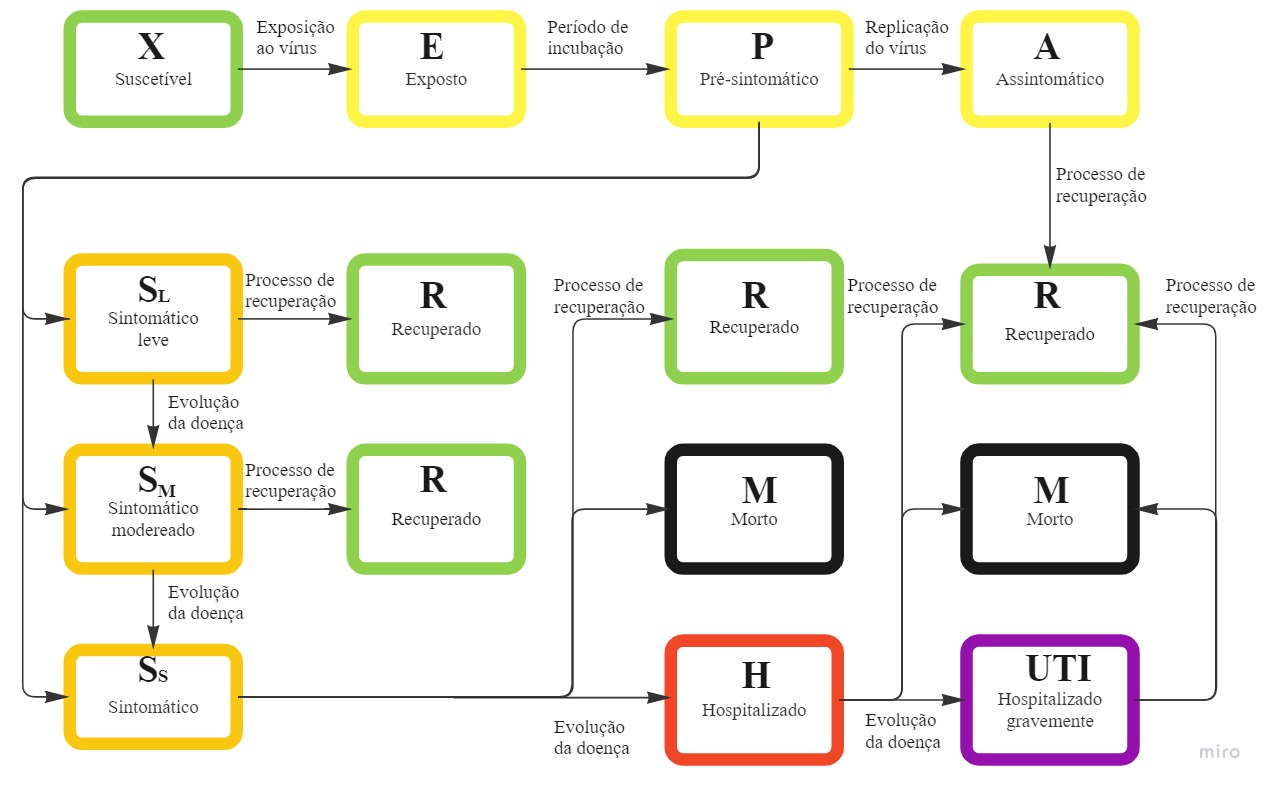
\includegraphics[width=0.9\textwidth]{Figures/covid fluxograma.jpg}
    \end{figure}

O indivíduo suscetível (X) entra em contato com o vírus e torna-se exposto (E), após o período de incubação torna-se pré-sintomático (P), a replicação do vírus ocorre e o indivíduo ou torna-se assintomático (A) e se recupera da doença, ou a doença evolui e o indivíduo se torna infeccioso, o indivíduo então pode ter sintomas leves ($S_l$), moderados ($S_m$) ou severos ($S_s$), caso não se recupere, será hospitalizado (H) e, em casos mais graves, internado em unidades de tratamento intensivo (UTI); na UTI o indivíduo ou se recupera, ou morre devido à doença.

No modelo, cada indivíduo ocupa uma posição em uma matriz quadrada de lado $L$ com população total $N = L \times L$, tal que $N$ é referente a cada cidade analisada. No início de cada simulação a população é iniciada com todos os indivíduos com estado suscetível (X), exceto 5 indivíduos que estarão em estado pré-sintomático, os indivíduos infectados entrarão em contato com sua vizinhança, Von Neumann para as cidades de baixa densidade populacional ou Moore para cidades de alta densidade, além dos contatos com outros indivíduos aleatórios. A probabilidade de infecção dos indivíduos suscetíveis é dada pela Equação \ref{eqn:prob}, um número aleatório $r$ é gerado e caso $r < P$, o indivíduo é infectado.

\section{Inicialização da população}

No início de cada simulação, além de receber o estado de saúde, cada indivíduo recebe uma idade atribuída de acordo com a estrutura etária da população brasileira, de modo que a distribuição de idades da rede reproduza a pirâmide etária real do país. A cada indivíduo é também atribuída uma idade de morte natural, sorteada por amostragem por rejeição a partir das probabilidades de morte natural por faixa etária, tal que a idade de morte respeita a expectativa de vida observada. Dessa forma, a rede inicia com uma população heterogênea em idade, o que é relevante uma vez que a evolução da Covid-19 e a sua letalidade dependem fortemente da faixa etária do indivíduo.

Os leitos de hospital e de UTI disponíveis para os doentes de Covid-19 são definidos a partir da razão de leitos por habitante de cada cidade, descontada a ocupação inicial de 50\% por outras doenças, de modo que apenas metade dos leitos esteja efetivamente disponível no início da simulação. A epidemia é iniciada com 5 indivíduos no estado pré-sintomático (P), distribuídos aleatoriamente na rede, enquanto os demais indivíduos permanecem suscetíveis.

\section{Dinâmica da simulação}

A simulação evolui em passos de tempo discretos, nos quais cada passo corresponde a um dia. A cada passo, antes de atualizar os estados, são aplicadas condições de contorno periódicas à rede, de modo que os indivíduos das bordas tenham como vizinhos os indivíduos da borda oposta, e logo a rede se comporta como uma superfície sem fronteiras, evitando efeitos de borda. Em seguida, percorre-se toda a rede e, para cada indivíduo, é aplicada a regra de transição correspondente ao seu estado de saúde atual, que determina o seu próximo estado. Por fim, a rede é atualizada de forma síncrona, ou seja, as transições calculadas para todos os indivíduos são aplicadas simultaneamente ao final do passo, de modo que a atualização de um indivíduo não interfira no cálculo dos demais no mesmo passo. O Algoritmo \ref{alg:simulacao} resume esse procedimento.

\begin{algorithm}[H]
\DontPrintSemicolon
\caption{Laço principal da simulação}
\label{alg:simulacao}
\For{cada simulação}{
  inicializa a população: estados de saúde, idades e leitos disponíveis\;
  \For{cada passo de tempo $t$ correspondente a um dia}{
    aplica as condições de contorno periódicas à rede\;
    \ForEach{indivíduo da rede}{
      aplica a regra de transição correspondente ao seu estado de saúde\;
    }
    atualiza a rede de forma síncrona\;
    substitui os indivíduos que sofreram morte natural por novos suscetíveis\;
    contabiliza a prevalência e a incidência de cada estado\;
  }
}
calcula a média das curvas sobre todas as simulações\;
\end{algorithm}

\subsection{Mecanismos de contágio}

A transmissão da doença ocorre por dois mecanismos complementares, ambos baseados na probabilidade de contágio dada pela Equação \ref{eqn:prob}. No primeiro mecanismo, cada indivíduo suscetível verifica a sua vizinhança e os seus contatos aleatórios, cujo número varia conforme a cidade, em busca de indivíduos infectados; o número de infectados encontrados, $n$, determina a probabilidade $P = 1 - (1 - \beta)^n$ de o suscetível ser infectado. No segundo mecanismo, cada indivíduo infectado, enquanto se encontra no período infeccioso, procura indivíduos suscetíveis entre seus contatos e tenta infectá-los, também de acordo com a probabilidade de contágio.

\begin{figure}[H]
\centering
\caption{Os dois mecanismos de contágio do modelo.}
\label{fig:contagio}
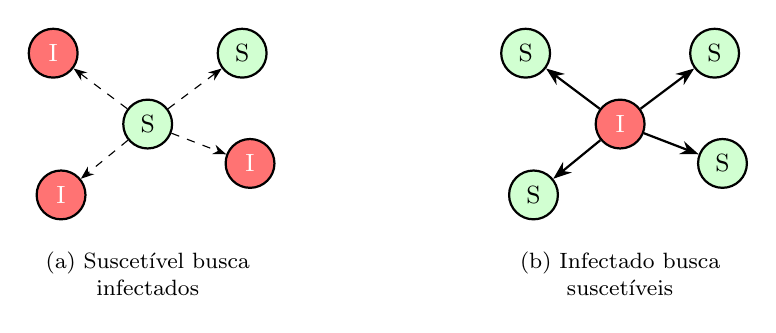
\begin{tikzpicture}[font=\small, >=Stealth,
   pessoa/.style={circle, draw, thick, minimum size=0.62cm, inner sep=0},
   susc/.style={pessoa, fill=green!18},
   infec/.style={pessoa, fill=red!55, text=white}]
  \begin{scope}
    \node[susc] (c1) at (0,0) {S};
    \node[infec] (a1) at (-1.2,0.9) {I};
    \node[susc]  (a2) at (1.2,0.9) {S};
    \node[infec] (a3) at (1.3,-0.5) {I};
    \node[infec] (a4) at (-1.1,-0.9) {I};
    \draw[->, dashed] (c1) -- (a1);
    \draw[->, dashed] (c1) -- (a2);
    \draw[->, dashed] (c1) -- (a3);
    \draw[->, dashed] (c1) -- (a4);
    \node[font=\footnotesize, align=center] at (0,-1.9) {(a) Suscetível busca\\ infectados};
  \end{scope}
  \begin{scope}[xshift=6cm]
    \node[infec] (c2) at (0,0) {I};
    \node[susc] (b1) at (-1.2,0.9) {S};
    \node[susc] (b2) at (1.2,0.9) {S};
    \node[susc] (b3) at (1.3,-0.5) {S};
    \node[susc] (b4) at (-1.1,-0.9) {S};
    \draw[->, thick] (c2) -- (b1);
    \draw[->, thick] (c2) -- (b2);
    \draw[->, thick] (c2) -- (b3);
    \draw[->, thick] (c2) -- (b4);
    \node[font=\footnotesize, align=center] at (0,-1.9) {(b) Infectado busca\\ suscetíveis};
  \end{scope}
\end{tikzpicture}
\end{figure}

Em (a), o indivíduo suscetível verifica a sua vizinhança e os seus contatos aleatórios em busca de infectados; em (b), o indivíduo infectado procura indivíduos suscetíveis entre seus contatos e tenta infectá-los. O segundo mecanismo é executado pelos estados pré-sintomático (P), assintomático (A) e sintomático leve ($S_l$), que representam os indivíduos infecciosos que ainda circulam na população, enquanto os estados sintomático moderado ($S_m$) e severo ($S_s$), por estarem afastados do convívio social, não procuram novos suscetíveis. Para evitar que um mesmo suscetível seja infectado duas vezes no mesmo passo de tempo, uma vez pela sua própria busca e outra por um infectado que o encontrou, utiliza-se um mecanismo de marcação que verifica se o indivíduo já foi contabilizado, garantindo a consistência da atualização.

\subsection{Transição entre estados e morte natural}

Cada estado de saúde possui uma duração, sorteada no momento em que o indivíduo entra no estado, dentro dos limites mínimo e máximo definidos para aquele estado (Tabela \ref{tab:dias}). Enquanto a duração não é atingida, o indivíduo permanece no mesmo estado; ao atingi-la, ocorre a transição para o próximo estado, que pode ser determinística ou sorteada de acordo com as probabilidades de transição (Tabela \ref{tab:prob}) e, em alguns casos, com a probabilidade de recuperação correspondente à faixa etária do indivíduo. A passagem para os estados de hospitalização (H) e de UTI depende ainda da disponibilidade de leitos, de modo que um indivíduo em estado severo só é hospitalizado se houver leito disponível.

Independentemente do estado de saúde, qualquer indivíduo pode sofrer morte natural ao atingir a sua idade de morte, situação na qual é removido e imediatamente substituído por um novo indivíduo suscetível, com idade sorteada novamente a partir da estrutura etária, de modo que o tamanho total da população permaneça constante ao longo da simulação.

\section{Parâmetros}

Para cada cidade a ser utilizada no modelo, a calibração da infecciosidade $\beta$ é necessária para que o valor de $R_0 = 3{,}5$ seja padrão em todas as cidades. É necessário também alterar os parâmetros que são específicos de cada cidade, são eles: tamanho da população, densidade populacional, contatos aleatórios, leitos de hospital e leitos de UTI, estes últimos obtidos a partir do Cadastro Nacional de Estabelecimentos de Saúde \cite{datasus}. A Tabela \ref{tab:area} mostra as características de quatro cidades: São Paulo (SP), Manaus (AM), Brasília (DF) e a favela da Rocinha (RJ).

\begin{table}[H]
\centering
\caption{Parâmetros de quatro diferentes áreas do Brasil.}
\label{tab:area}
\begin{tabular}{l c c c c c}
\hline
\textbf{Área} & \textbf{Densidade} & \textbf{L} & \textbf{Leitos/Pop} & \textbf{UTI/Pop} & \textbf{Contatos} \\
\hline
São Paulo & Alta  & 3355 & 0,00247452 & 0,00043782 & 2--19 \\
Rocinha   & Alta  & 264  & 0,00055111 & 0,00014592 & 2--120 \\
Brasília  & Baixa & 1604 & 0,00260879 & 0,00040114 & 2 \\
Manaus    & Baixa & 1343 & 0,00187124 & 0,00027858 & 2 \\
\hline
\end{tabular}
\end{table}

Já os parâmetros relacionados à doença são comuns a todas as áreas modeladas. A Tabela \ref{tab:dias} mostra a duração, em dias, do período de cada estado de saúde, e a Tabela \ref{tab:prob} mostra a probabilidade de transição entre os estados de saúde.

\begin{table}[H]
\centering
\caption{Parâmetros de duração de cada estado de saúde.}
\label{tab:dias}
\begin{tabular}{l l c}
\hline
\textbf{Parâmetro} & \textbf{Descrição} & \textbf{Duração (dias)} \\
\hline
$\tau_{l}$    & Período de latência   & 0--27 \\
$\tau_{P}$    & Pré-sintomático       & 0--14 \\
$\tau_{A}$    & Assintomático         & 0--7  \\
$\tau_{S_l}$  & Sintomático leve      & 0--14 \\
$\tau_{S_m}$  & Sintomático moderado  & 0--28 \\
$\tau_{S_s}$  & Sintomático severo    & 0--4  \\
$\tau_{H}$    & Hospitalização        & 7--45 \\
$\tau_{UTI}$  & UTI                   & 10--60 \\
\hline
\end{tabular}
\end{table}

\begin{table}[H]
\centering
\caption{Probabilidades de transição entre estados de saúde.}
\label{tab:prob}
\begin{tabular}{l l c}
\hline
\textbf{Parâmetro} & \textbf{Transição entre estados} & \textbf{Probabilidade} \\
\hline
$P_{(P\rightarrow A)}$    & Pré-sintomático para assintomático        & 0,5  \\
$P_{(P\rightarrow S_l)}$  & Pré-sintomático para sintomático leve     & 0,6  \\
$P_{(P\rightarrow S_m)}$  & Pré-sintomático para sintomático moderado & 0,2  \\
$P_{(P\rightarrow S_s)}$  & Pré-sintomático para sintomático severo   & 0,2  \\
$P_{(S_l\rightarrow S_m)}$ & Sintomático leve para sintomático moderado & 0,1 \\
$P_{(S_s\rightarrow H)}$   & Sintomático severo para hospitalização    & 0,75 \\
$P_{(S_s\rightarrow UTI)}$ & Sintomático severo para internação em UTI & 0,25 \\
\hline
\end{tabular}
\end{table}

\section{Estratégia de paralelização e validação}

A estratégia de paralelização adotada baseia-se no paralelismo de dados: uma vez que, a cada passo de tempo, todos os indivíduos da rede são processados de forma independente, associa-se uma thread a cada indivíduo, de modo que toda a rede é processada simultaneamente. A dinâmica da simulação é decomposta em kernels, um para cada estado de saúde, lançados em sequência a cada passo; como o lançamento de cada kernel funciona como um ponto de sincronização global, a ordem em que os estados são tratados na implementação serial é preservada. A geração de números aleatórios, por sua vez, é adaptada para a execução paralela, atribuindo-se um estado de gerador a cada thread. Em todas essas decisões, o princípio orientador é a preservação do comportamento do modelo, de modo que a implementação paralela reproduza os resultados da implementação serial.

Para que a paralelização seja considerada bem-sucedida, não basta que seja mais rápida; é necessário que produza os mesmos resultados da implementação serial, tomada como referência. A validação é feita comparando-se as curvas epidêmicas obtidas pelas duas implementações sob os mesmos parâmetros (mesma infecciosidade $\beta$, mesmo tamanho de rede e mesmo número de simulações), para cada uma das cidades modeladas. A concordância entre as curvas é quantificada pelo erro quadrático médio entre as proporções de cada estado ao longo do tempo, de modo que uma diferença pequena, compatível com a flutuação estatística do método de Monte Carlo, indica a equivalência entre as implementações.

Confirmada a equivalência, avalia-se o ganho de desempenho da implementação paralela. A avaliação é feita medindo-se a aceleração, definida no Capítulo \ref{FT} como a razão entre o tempo de execução da implementação serial e o da implementação paralela, e a eficiência correspondente, para cada cidade. Como as cidades possuem tamanhos de rede distintos, essa avaliação permite ainda observar como o ganho de desempenho varia com o tamanho do problema. A Figura \ref{fig:estrategia} resume a estratégia do trabalho.

\begin{figure}[H]
\centering
\caption{Estratégia do trabalho.}
\label{fig:estrategia}
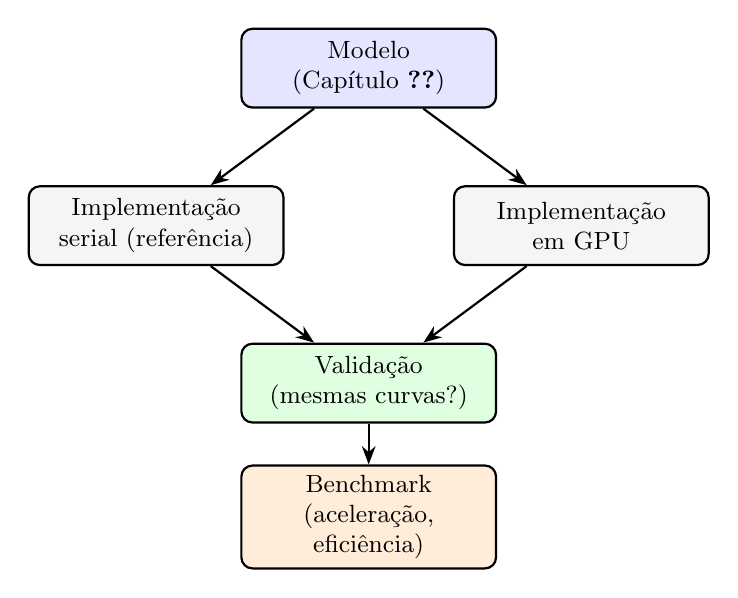
\begin{tikzpicture}[font=\small, >=Stealth,
   bx/.style={draw, thick, rounded corners, align=center, minimum height=1cm, text width=3cm, fill=gray!8}]
  \node[bx, fill=blue!10] (modelo) at (0,0) {Modelo\\ (Capítulo \ref{Met})};
  \node[bx] (serial) at (-2.7,-2) {Implementação\\ serial (referência)};
  \node[bx] (gpu) at (2.7,-2) {Implementação\\ em GPU};
  \node[bx, fill=green!12] (valid) at (0,-4) {Validação\\ (mesmas curvas?)};
  \node[bx, fill=orange!15] (bench) at (0,-5.7) {Benchmark\\ (aceleração, eficiência)};
  \draw[->, thick] (modelo) -- (serial);
  \draw[->, thick] (modelo) -- (gpu);
  \draw[->, thick] (serial) -- (valid);
  \draw[->, thick] (gpu) -- (valid);
  \draw[->, thick] (valid) -- (bench);
\end{tikzpicture}
\end{figure}

O mesmo modelo é realizado em duas implementações; a implementação em GPU é validada contra a serial sob os mesmos parâmetros e, confirmada a equivalência, avalia-se o seu desempenho.

%=============================================================
\chapter{Implementação serial}
\label{cap:serial}
%=============================================================

A implementação serial do modelo, escrita na linguagem C, constitui a referência deste trabalho, uma vez que é contra os seus resultados que a implementação paralela será validada. Neste capítulo descreve-se como o modelo apresentado no Capítulo \ref{Met} é realizado como um programa sequencial, no qual um único processador percorre toda a rede a cada passo de tempo.

\section{Estrutura de dados}

Cada indivíduo da população é representado por uma estrutura que reúne o seu estado de saúde e os atributos necessários à evolução da doença, e a rede é representada por uma matriz dessas estruturas. A Listagem \ref{lst:struct} apresenta os principais campos dessa estrutura.

\begin{lstlisting}[caption={Estrutura que representa cada indivíduo (agente).}, label={lst:struct}]
struct Individual {
    int Health;        // estado de saúde atual
    int Swap;          // próximo estado (atualização síncrona)
    int AgeYears;      // idade em anos
    int AgeDays;       // idade em dias
    int AgeDeathYears; // idade de morte natural (anos)
    int AgeDeathDays;  // idade de morte natural (dias)
    int StateTime;     // duração sorteada para o estado atual
    int TimeOnState;   // tempo já decorrido no estado atual
    int Days;          // dias do indivíduo na simulação
    int Isolation;     // indicador de isolamento
    int Exponent;      // tentativas de infecção no passo
    int Checked;       // marca para evitar dupla infecção
} Person[L+2][L+2];
\end{lstlisting}

O campo \texttt{Health} armazena o estado de saúde atual do indivíduo, enquanto o campo \texttt{Swap} armazena o estado para o qual ele transitará, mecanismo detalhado adiante. Os campos de idade guardam a idade atual e a idade de morte natural do indivíduo, e os campos \texttt{StateTime} e \texttt{TimeOnState} guardam, respectivamente, a duração sorteada para o estado atual e o tempo já decorrido nesse estado, de modo que a transição ocorre quando \texttt{TimeOnState} atinge \texttt{StateTime}. Por fim, os campos \texttt{Exponent} e \texttt{Checked} são utilizados no controle do contágio, evitando que um mesmo suscetível seja infectado mais de uma vez no mesmo passo.

A rede é declarada como uma matriz \texttt{Person[L+2][L+2]}, na qual as duas linhas e as duas colunas adicionais formam uma borda que armazena cópias das extremidades opostas da rede, implementando as condições de contorno periódicas descritas no Capítulo \ref{Met}; dessa forma, ao verificar a vizinhança de um indivíduo da borda, o programa encontra automaticamente os vizinhos da borda oposta.

A atualização da rede é feita de forma síncrona por meio de um duplo-buffer, no qual os campos \texttt{Health} e \texttt{Swap} desempenham papéis complementares. Durante a varredura da rede, as funções de estado leem o estado atual de cada indivíduo em \texttt{Health} e escrevem o seu próximo estado em \texttt{Swap}, sem alterar \texttt{Health}; somente ao final do passo o conteúdo de \texttt{Swap} é copiado para \texttt{Health}. Assim, garante-se que a atualização de um indivíduo não interfira no cálculo dos demais no mesmo passo, conforme ilustra a Figura \ref{fig:duplobuffer}.

\begin{figure}[H]
\centering
\caption{Duplo-buffer da atualização síncrona.}
\label{fig:duplobuffer}
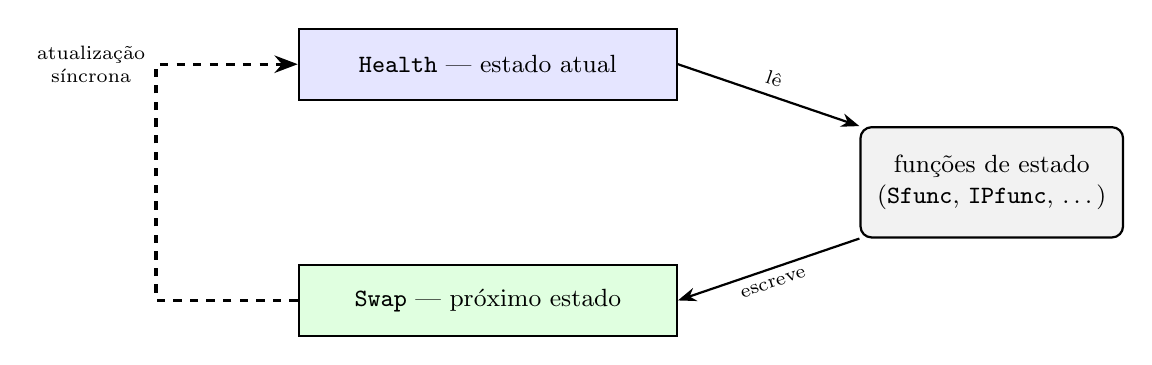
\begin{tikzpicture}[font=\small, >=Stealth]
  \node[draw, thick, fill=blue!10, minimum width=4.8cm, minimum height=0.9cm] (health) at (0,1.5) {\texttt{Health} --- estado atual};
  \node[draw, thick, fill=green!12, minimum width=4.8cm, minimum height=0.9cm] (swap) at (0,-1.5) {\texttt{Swap} --- próximo estado};
  \node[draw, thick, rounded corners, fill=gray!10, align=center, text width=3.1cm, minimum height=1.4cm] (func) at (6.4,0) {funções de estado\\ (\texttt{Sfunc}, \texttt{IPfunc}, \dots)};
  \draw[->, thick] (health.east) -- (func.north west) node[midway, above, sloped, font=\scriptsize]{lê};
  \draw[->, thick] (func.south west) -- (swap.east) node[midway, below, sloped, font=\scriptsize]{escreve};
  \draw[->, very thick, dashed] (swap.west) -- ++(-1.8,0) |- (health.west) node[pos=0.5, left, align=center, font=\scriptsize]{atualização\\ síncrona};
\end{tikzpicture}
\end{figure}

Durante a varredura, as funções de estado leem o estado atual em \texttt{Health} e escrevem o próximo estado em \texttt{Swap}; ao final do passo, \texttt{Swap} é copiado para \texttt{Health}, de modo que todas as transições de um passo são aplicadas simultaneamente.

\section{Organização do programa e geração de números aleatórios}

O programa é organizado de forma modular, no qual o arquivo principal contém o laço de simulação e inclui diversos arquivos auxiliares, cada um responsável por uma parte do modelo: a inicialização da população, os parâmetros de cada cidade, as probabilidades de morte natural e de recuperação por faixa etária, os dois mecanismos de contágio e as funções de estado. Cada estado de saúde possui a sua própria função, o que mantém o código legível e preserva a correspondência direta entre o modelo e a sua implementação.

Como o modelo é estocástico, a geração de números aleatórios é parte essencial da implementação. Utiliza-se um gerador congruencial linear multiplicativo, apresentado na Listagem \ref{lst:rng}, no qual o estado do gerador é multiplicado por uma constante a cada chamada e normalizado para o intervalo $[0,1]$. A cada simulação o gerador é inicializado com uma semente distinta, derivada do número da simulação, de modo que cada simulação produz uma sequência própria de números pseudoaleatórios e, ao mesmo tempo, os resultados permanecem reprodutíveis.

\begin{lstlisting}[caption={Gerador congruencial linear multiplicativo.}, label={lst:rng}]
double aleat() {
    R *= mult;                // mult = 888121
    rn = (double) R / MAXNUM; // número em [0, 1]
}
\end{lstlisting}

\section{Inicialização da população}

Antes do início do laço de simulação, a função de inicialização prepara a população de acordo com o descrito no Capítulo \ref{Met}. Toda a rede é colocada no estado suscetível e, a cada indivíduo, é atribuída uma idade sorteada a partir da estrutura etária brasileira, bem como uma idade de morte natural obtida por amostragem por rejeição sobre as probabilidades de morte por faixa etária. Em seguida, os 5 casos iniciais são posicionados aleatoriamente na rede no estado pré-sintomático. A Listagem \ref{lst:begin} apresenta a estrutura dessa função.

\begin{lstlisting}[caption={Inicialização da população (\texttt{beginfunc}).}, label={lst:begin}]
void beginfunc() {
    for (i = 1; i <= L; i++)
      for (j = 1; j <= L; j++) {
        Person[i][j].Health = S;            // toda a rede em suscetível

        // sorteia a faixa etária pela estrutura etária e a idade na faixa
        Person[i][j].AgeYears = rn * (MaximumAge - MinimumAge) + MinimumAge;
        aleat();
        Person[i][j].AgeDays  = rn * 365;

        // idade de morte natural por amostragem por rejeição
        do {
            aleat(); Person[i][j].AgeDeathYears = rn * 100;
            aleat();
        } while (rn >= ProbNaturalDeath[Person[i][j].AgeDeathYears]);
        Person[i][j].AgeDeathDays = Person[i][j].AgeDeathYears * 365;
      }

    // distribui os IPini = 5 casos iniciais em posições aleatórias
    for (k = 0; k < IPini; ) {
        aleat(); i = rn * L + 1;
        aleat(); j = rn * L + 1;
        if (Person[i][j].Health == S) {
            Person[i][j].Health = IP;
            aleat();
            Person[i][j].StateTime = rn * (MaxIP - MinIP) + MinIP;
            k++;
        }
    }
}
\end{lstlisting}

\section{Laço de simulação e funções de estado}

O laço principal segue o procedimento descrito no Algoritmo \ref{alg:simulacao}. Para cada simulação, a população é inicializada e, em seguida, a simulação avança dia a dia: a cada passo, as condições de contorno periódicas são aplicadas e a rede é percorrida sequencialmente, de modo que, para cada indivíduo, é chamada a função correspondente ao seu estado de saúde atual. Concluída a varredura, a rede é atualizada. A Listagem \ref{lst:loop} apresenta esse laço, no qual \texttt{estado\_IS}($\cdot$) abrevia o teste dos estados sintomáticos (IA, $S_l$, $S_m$ e $S_s$).

\begin{lstlisting}[caption={Laço principal: contorno periódico, varredura e atualização.}, label={lst:loop}]
for (sim_time = 0; sim_time <= DAYS; sim_time++) {
    // condições de contorno periódicas (bordas e cantos)
    for (i = 1; i <= L; i++) {
        Person[0][i].Health   = Person[L][i].Health;
        Person[L+1][i].Health = Person[1][i].Health;
        Person[i][0].Health   = Person[i][L].Health;
        Person[i][L+1].Health = Person[i][1].Health;
    }

    // varredura da rede: despacho por estado de saúde
    for (i = 1; i <= L; i++)
      for (j = 1; j <= L; j++)
        if      (Person[i][j].Health == S)   Sfunc(i, j);
        else if (Person[i][j].Health == E)   Efunc(i, j);
        else if (Person[i][j].Health == IP)  IPfunc(i, j);
        else if (estado_IS(Person[i][j].Health)) ISfunc(i, j);
        else if (Person[i][j].Health == H)   Hfunc(i, j);
        else if (Person[i][j].Health == ICU) ICUfunc(i, j);

    Updatefunc();   // atualização síncrona
}
\end{lstlisting}

Cada função de estado segue uma estrutura semelhante: incrementa o tempo decorrido no estado, verifica se o indivíduo sofreu morte natural e, caso contrário, decide a sua permanência ou transição. Enquanto o tempo decorrido não atinge a duração sorteada, o indivíduo permanece no mesmo estado; ao atingi-la, a função sorteia o próximo estado de acordo com as probabilidades de transição e, quando aplicável, com a probabilidade de recuperação correspondente à sua faixa etária, escrevendo o resultado no campo \texttt{Swap}. As funções dos estados infecciosos que ainda circulam na população acrescentam, enquanto o indivíduo permanece infeccioso, a chamada ao segundo mecanismo de contágio, descrito a seguir. A Listagem \ref{lst:ipfunc} ilustra essa estrutura para o estado pré-sintomático.

\begin{lstlisting}[caption={Função de estado do pré-sintomático (\texttt{IPfunc}).}, label={lst:ipfunc}]
void IPfunc(int i, int j) {
    Person[i][j].TimeOnState++;

    if (Person[i][j].Days >= Person[i][j].AgeDeathDays) {   // morte natural
        Person[i][j].Swap = Dead;
        New_Dead++;
    }
    else if (Person[i][j].TimeOnState >= Person[i][j].StateTime) {
        // duração do estado terminou: sorteia o próximo estado
        aleat();
        if (rn < ProbIPtoIA) {
            Person[i][j].Swap = IA;
            aleat();
            Person[i][j].StateTime = rn * (MaxIA - MinIA) + MinIA;
        } else {
            // sorteia ISLight / ISModerate / ISSevere conforme as probabilidades
            // ...
        }
    }
    else {                            // ainda infeccioso
        Neighborsinfectedfunc(i, j);  // segundo mecanismo de contágio
        Person[i][j].Swap = IP;
    }
}
\end{lstlisting}

As funções dos estados sintomático severo, hospitalizado e de UTI consideram ainda a disponibilidade de leitos: um indivíduo em estado severo só é hospitalizado se houver leito de hospital disponível, e a internação em UTI depende da disponibilidade de leitos de UTI. O número de leitos disponíveis em cada cidade desconta a ocupação inicial por outras doenças, conforme descrito no Capítulo \ref{Met}, e é controlado por contadores atualizados ao longo da simulação.

\section{Implementação dos mecanismos de contágio}

O primeiro mecanismo de contágio é realizado pela função associada ao estado suscetível, que percorre a vizinhança local do indivíduo --- de Moore para as cidades de alta densidade e de Von Neumann para as de baixa densidade --- e os seus contatos aleatórios, contando o número $n$ de indivíduos infectados encontrados. A partir desse número, calcula-se a probabilidade de contágio $P = 1 - (1 - \beta)^n$ e, com um número aleatório, decide-se se o suscetível é infectado, caso em que ele transita para o estado exposto. A Listagem \ref{lst:neighbors} apresenta esse mecanismo, no qual \texttt{infeccioso}($\cdot$) denota o teste de o indivíduo estar em um estado infeccioso.

\begin{lstlisting}[caption={Primeiro mecanismo: o suscetível busca infectados (\texttt{Neighborsfunc}).}, label={lst:neighbors}]
int Neighborsfunc(int i, int j) {
    int KI = 0;            // número de infectados encontrados
    Contagion = 0;

    if (Person[i][j].Isolation == IsolationNo) {   // contatos aleatórios
        aleat();
        RandomContacts = rn * (MaxRandomContacts - MinRandomContacts) + MinRandomContacts;
        for (mute = 0; mute < RandomContacts; mute++) {
            // sorteia um contato (Randomi, Randomj)
            if (infeccioso(Randomi, Randomj)) KI++;
        }
    }

#if (Density == HIGH)              // vizinhança de Moore (8 vizinhos)
    for (k = -1; k <= 1; k++)
      for (l = -1; l <= 1; l++)
        if (infeccioso(i + k, j + l)) KI++;
#else                              // vizinhança de Von Neumann (4 vizinhos)
    if (infeccioso(i-1,j) || infeccioso(i+1,j) ||
        infeccioso(i,j-1) || infeccioso(i,j+1)) KI++;
#endif

    if (KI > 0) {                  // P = 1 - (1 - Beta)^KI
        ProbContagion = 1.0 - pow(1.0 - Beta, (double) KI);
        aleat();
        if (rn <= ProbContagion) Contagion = 1;
    }
    return Contagion;
}
\end{lstlisting}

O segundo mecanismo é realizado pelos indivíduos infecciosos que ainda circulam na população, que procuram indivíduos suscetíveis entre seus contatos aleatórios e tentam infectá-los. Para garantir a consistência com a atualização síncrona e evitar que um mesmo suscetível seja infectado duas vezes no mesmo passo, cada suscetível dispõe dos campos \texttt{Exponent} e \texttt{Checked}: o primeiro contabiliza as tentativas de infecção dirigidas àquele indivíduo no passo, enquanto o segundo marca o indivíduo já processado, de modo que a infecção é aplicada uma única vez por passo, independentemente de ter origem na busca do próprio suscetível ou na de um infectado. A Listagem \ref{lst:neighborsinf} apresenta esse mecanismo.

\begin{lstlisting}[caption={Segundo mecanismo: o infectado busca suscetíveis (\texttt{Neighborsinfectedfunc}).}, label={lst:neighborsinf}]
void Neighborsinfectedfunc(int i, int j) {
    if (Person[i][j].Isolation == IsolationNo) {
        aleat();
        RandomContacts = rn * (MaxRandomContacts - MinRandomContacts) + MinRandomContacts;
        for (mute = 0; mute < RandomContacts; mute++) {
            // sorteia um suscetível-alvo (Randomi, Randomj)
            if (Person[Randomi][Randomj].Health == S)
                Person[Randomi][Randomj].Exponent++;

            if (Person[Randomi][Randomj].Checked == 0 &&
                Person[Randomi][Randomj].Exponent == 1) {
                ProbContagion = 1.0 - pow(1.0 - Beta, (double) Person[Randomi][Randomj].Exponent);
                aleat();
                if (rn <= ProbContagion) {
                    Person[Randomi][Randomj].Checked = 1;
                    Person[Randomi][Randomj].Swap = E;
                    Person[Randomi][Randomj].TimeOnState = 0;
                    aleat();
                    Person[Randomi][Randomj].StateTime = rn * (MaxLatency - MinLatency) + MinLatency;
                }
            }
        }
    }
}
\end{lstlisting}

\section{Atualização síncrona e geração das saídas}

Ao final de cada passo de tempo, a função de atualização copia o campo \texttt{Swap} para o campo \texttt{Health} de todos os indivíduos, efetivando de forma síncrona as transições calculadas durante a varredura, e incrementa os contadores de idade e de tempo de simulação. Em seguida, contabiliza-se quantos indivíduos se encontram em cada estado de saúde, e os indivíduos que atingiram a sua idade de morte natural são removidos e substituídos por novos suscetíveis, com idade sorteada novamente a partir da estrutura etária, de modo que o tamanho total da população permanece constante. A Listagem \ref{lst:update} apresenta o trecho central dessa atualização.

\begin{lstlisting}[caption={Atualização síncrona e substituição dos mortos (\texttt{Updatefunc}).}, label={lst:update}]
for (i = 1; i <= L; i++)
  for (j = 1; j <= L; j++) {
    Person[i][j].Health = Person[i][j].Swap;   // atualização síncrona
    Person[i][j].Exponent = 0;
    Person[i][j].Checked  = 0;
    Person[i][j].AgeDays++;
    Person[i][j].Days++;

    if (Person[i][j].Health == Dead || Person[i][j].Health == DeadCovid) {
        Person[i][j].Health = S;                // novo suscetível
        aleat();
        Person[i][j].AgeYears = rn * 100;       // idade reamostrada
        // ... sorteia a idade de morte natural (amostragem por rejeição)
    }
  }
\end{lstlisting}

Os resultados são registrados em dois níveis. Para cada simulação, a prevalência e a incidência de cada estado de saúde são gravadas, a cada dia, em arquivos próprios. Ao final de todas as simulações, calcula-se a média das curvas sobre as \texttt{MAXSIM} simulações, obtendo-se, pelo método de Monte Carlo, as curvas médias de prevalência e de incidência que representam a evolução esperada da epidemia.

%=============================================================
\chapter{Implementação em GPU}
\label{cap:gpu}
%=============================================================

A implementação paralela do modelo em CUDA constitui a principal contribuição deste trabalho. O mesmo modelo descrito no Capítulo \ref{Met} e a mesma lógica da implementação serial são reorganizados de modo que a rede seja processada em paralelo, com uma thread responsável por cada indivíduo. O desafio central é preservar o comportamento do modelo --- e, portanto, a equivalência com o serial --- ao mesmo tempo em que se explora o paralelismo da GPU.

\section{Mapeamento da rede em threads}

Na implementação serial, um único processador percorre a rede com dois laços encaixados e, para cada indivíduo, despacha a função correspondente ao seu estado. Na GPU, esse percurso sequencial dá lugar ao paralelismo: a cada indivíduo é associada uma thread, de modo que toda a rede é processada simultaneamente. Como a rede possui $(L+2)^2$ posições, são lançadas $(L+2)^2$ threads, organizadas em blocos de tamanho fixo; cada thread identifica a sua posição a partir dos índices nativos de CUDA e converte esse índice linear na posição $(i, j)$ da matriz, ignorando as células da borda. A Listagem \ref{lst:idx} apresenta as funções de conversão entre o índice da thread e a posição na rede.

\begin{lstlisting}[caption={Conversão entre o índice da thread e a posição na rede.}, label={lst:idx}]
__host__ __device__ int to1D(int i, int j, int L) {
    return i * (L + 2) + j;
}
__host__ __device__ void to2D(int idx, int L, int &i, int &j) {
    i = idx / (L + 2);
    j = idx % (L + 2);
}
\end{lstlisting}

Outra diferença em relação ao serial está no tratamento dos estados de saúde. Em vez de uma única varredura com um despacho condicional, cada estado possui o seu próprio kernel, lançado sobre toda a rede: cada thread verifica se o seu indivíduo se encontra no estado tratado por aquele kernel e, em caso afirmativo, aplica a regra correspondente. Os kernels de estado são lançados em sequência a cada dia --- contorno, S, E, IP, IS, H, UTI e atualização ---; uma vez que o lançamento de cada kernel é um ponto de sincronização global, a ordem das funções de estado do serial é preservada, o que é essencial para a equivalência entre as implementações.

\section{Estrutura de dados na GPU}

Cada indivíduo é representado na GPU por uma estrutura análoga à do serial, alinhada em 16 bytes para favorecer o acesso à memória, e a rede é armazenada como um vetor dessas estruturas na memória global do \textit{device}. Os parâmetros do modelo --- a infecciosidade, os parâmetros de cada cidade, as durações dos estados e os códigos dos estados de saúde --- são armazenados em memória constante, apropriada para dados apenas de leitura que são acessados por todas as threads. A Listagem \ref{lst:gpustruct} apresenta a estrutura e alguns desses parâmetros.

\begin{lstlisting}[caption={Estrutura do indivíduo e parâmetros em memória constante.}, label={lst:gpustruct}]
struct __align__(16) GPUPerson {
    int Health, Swap, Gender;
    int AgeYears, AgeDays, AgeDeathYears, AgeDeathDays;
    int StateTime, TimeOnState, Days;
    int Isolation, Exponent, Checked;
};

// parâmetros e códigos de estado em memória constante
__constant__ double d_Beta;
__constant__ int    d_Density;
__constant__ double d_MaxRandomContacts, d_MinRandomContacts;
__constant__ int    d_S, d_E, d_IP, d_IA, d_ISLight, d_ISModerate, d_ISSevere;

// vetor compacto de Health (1 byte por célula)
__device__ unsigned char* d_HealthC;
\end{lstlisting}

\subsection{Otimização da estrutura de Health}

Os mecanismos de contágio percorrem, para cada indivíduo, diversos contatos aleatórios espalhados pela rede, lendo de cada um apenas o seu estado de saúde. Como cada estrutura completa ocupa aproximadamente 52 bytes, esses acessos aleatórios a posições distantes da memória são pouco eficientes e, para redes grandes, ultrapassam a capacidade da cache. Para contornar essa limitação, mantém-se um vetor compacto que replica apenas o campo de estado de saúde, com um byte por célula, conforme ilustra a Figura \ref{fig:healthsoa}. Os mecanismos de contágio leem desse vetor compacto, de modo que o conjunto de dados percorrido pelos acessos aleatórios é pequeno o suficiente para permanecer na cache L2 (Capítulo \ref{FT}), o que reduz o tempo gasto com acesso à memória, fator determinante para o desempenho. O vetor compacto é mantido sincronizado com o estado de saúde ao final de cada atualização.

\begin{figure}[htb]
\centering
\caption{Otimização da estrutura de Health.}
\label{fig:healthsoa}
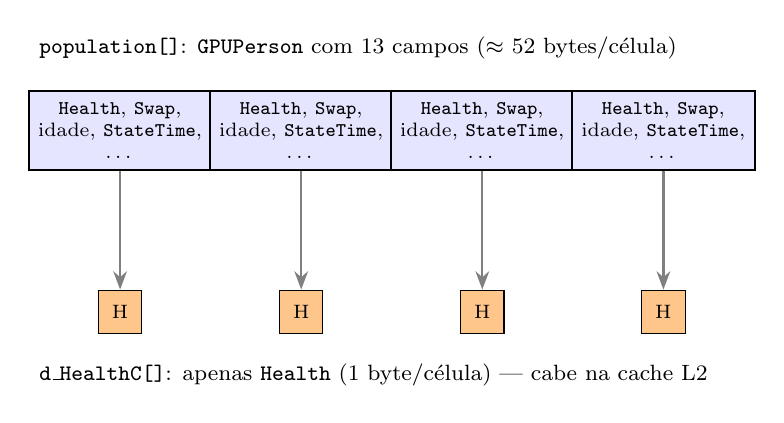
\begin{tikzpicture}[font=\small, >=Stealth]
  \foreach \x in {0,1,2,3} {
    \node[draw, thick, fill=blue!10, minimum width=2.1cm, minimum height=1.0cm, align=center, font=\scriptsize] (p\x) at (\x*2.3,0) {\texttt{Health}, \texttt{Swap},\\ idade, \texttt{StateTime},\\ \dots};
    \node[draw, fill=orange!45, minimum width=0.55cm, minimum height=0.55cm, font=\scriptsize] (c\x) at (\x*2.3,-2.3) {H};
    \draw[->, thick, gray] (p\x.south) -- (c\x.north);
  }
  \node[anchor=west, font=\footnotesize] at (-1.15,1.05) {\texttt{population[]}: \texttt{GPUPerson} com 13 campos ($\approx$ 52 bytes/célula)};
  \node[anchor=west, font=\footnotesize] at (-1.15,-3.1) {\texttt{d\_HealthC[]}: apenas \texttt{Health} (1 byte/célula) --- cabe na cache L2};
\end{tikzpicture}
\source{O autor.}
\end{figure}

O vetor completo \texttt{population[]} armazena todos os campos de cada indivíduo; o vetor compacto \texttt{d\_HealthC[]} replica apenas o campo \texttt{Health}, de modo que os acessos aleatórios dos mecanismos de contágio percorrem um vetor pequeno o suficiente para permanecer na cache L2.

\section{Geração de números aleatórios thread-safe}

A geração de números aleatórios do serial utiliza um único estado global, avançado a cada chamada, o que é incompatível com a execução paralela, uma vez que diversas threads o acessariam simultaneamente, introduzindo condições de corrida. Na implementação em GPU, mantém-se um vetor de estados, um por thread, e cada thread avança apenas o seu próprio estado, utilizando o mesmo gerador congruencial linear multiplicativo do serial. Cada estado é inicializado com uma semente própria, derivada do índice da thread, de modo que as threads produzem sequências independentes, sem condições de corrida, e os resultados permanecem reprodutíveis. A Listagem \ref{lst:gpurng} apresenta o gerador e a sua inicialização.

\begin{lstlisting}[caption={Gerador de números aleatórios por thread.}, label={lst:gpurng}]
__device__ double generateRandom(unsigned int* state) {
    unsigned long long t = (unsigned long long)(*state) * 888121ULL;
    *state = (unsigned int)(t & 0xFFFFFFFF);   // mantém 32 bits, como no serial
    return (double)(*state) / 4294967295.0;
}

__global__ void initRNG(unsigned int* states, unsigned int seed, int size) {
    int idx = blockIdx.x * blockDim.x + threadIdx.x;
    if (idx < size)
        states[idx] = seed * (idx + 1);        // semente única por thread
}
\end{lstlisting}

\section{Inicialização e laço de simulação}

A orquestração da simulação é feita pelo \textit{host}, que aloca a memória do \textit{device}, executa o laço sobre as simulações e, em cada simulação, inicializa os estados do gerador, a população e os casos iniciais. A inicialização da população é realizada em paralelo por um kernel, no qual cada thread coloca o seu indivíduo no estado suscetível e sorteia a sua idade e a sua idade de morte natural, e os 5 casos iniciais são posicionados em seguida. A cada dia, o \textit{host} lança a sequência de kernels que constitui um passo da simulação, conforme apresenta a Listagem \ref{lst:rundia}. Ao final de todas as simulações, os contadores são copiados do \textit{device} para o \textit{host}, que calcula a média das curvas sobre as simulações, do mesmo modo que na implementação serial.

\begin{lstlisting}[caption={Sequência de kernels lançada a cada dia.}, label={lst:rundia}]
void runSimulationDay(GPUPerson* d_pop, unsigned int* d_rng,
                      int L, int day, int blockSize, int numBlocks) {
    updateBoundaries_kernel <<<numBlocks, blockSize>>> (d_pop, L);
    S_kernel   <<<numBlocks, blockSize>>> (d_pop, d_rng, L);
    E_kernel   <<<numBlocks, blockSize>>> (d_pop, d_rng, L);
    IP_kernel  <<<numBlocks, blockSize>>> (d_pop, d_rng, L);
    IS_kernel  <<<numBlocks, blockSize>>> (d_pop, d_rng, L);
    H_kernel   <<<numBlocks, blockSize>>> (d_pop, d_rng, L);
    ICU_kernel <<<numBlocks, blockSize>>> (d_pop, d_rng, L);
    update_kernel <<<numBlocks, blockSize>>> (d_pop, d_rng, L, day, d_ProbNaturalDeath);
}
\end{lstlisting}

\section{Mecanismos de contágio em paralelo}

O primeiro mecanismo é realizado pelo kernel do estado suscetível: cada thread cujo indivíduo é suscetível verifica a sua vizinhança e os seus contatos aleatórios, conta os infectados encontrados e, a partir da probabilidade de contágio, decide se o indivíduo passa ao estado exposto. A Listagem \ref{lst:skernel} apresenta esse kernel.

\begin{lstlisting}[caption={Primeiro mecanismo: kernel do estado suscetível.}, label={lst:skernel}]
__global__ void S_kernel(GPUPerson* population, unsigned int* rngStates, int L) {
    int idx = blockIdx.x * blockDim.x + threadIdx.x;
    if (idx >= (L + 2) * (L + 2)) return;

    int i, j;
    to2D(idx, L, i, j);
    if (i < 1 || i > L || j < 1 || j > L) return;   // ignora a borda

    int p = to1D(i, j, L);
    if (population[p].Health != d_S) return;

    if (population[p].Days >= population[p].AgeDeathDays) {   // morte natural
        population[p].Swap = d_Dead;
        return;
    }
    // busca infectados na vizinhança e nos contatos aleatórios
    ContactResult c = checkAllContacts(i, j, L, population, &rngStates[idx]);
    if (c.anyContact &&
        generateRandom(&rngStates[idx]) <= calculateInfectionProbability(c.infectiousContacts)) {
        population[p].Checked = 1;
        population[p].Swap = d_E;
        population[p].TimeOnState = 0;
        population[p].StateTime =
            generateRandom(&rngStates[idx]) * (d_MaxLatency - d_MinLatency) + d_MinLatency;
    } else {
        population[p].Swap = d_S;
    }
}
\end{lstlisting}

O segundo mecanismo é realizado por uma função executada pelos kernels dos estados pré-sintomático, assintomático e sintomático leve, enquanto o indivíduo permanece infeccioso: a função sorteia contatos aleatórios e tenta infectar os suscetíveis encontrados. Aqui surge o principal cuidado da paralelização: como diversas threads de indivíduos infectados podem mirar o mesmo suscetível simultaneamente, o incremento simples do campo \texttt{Exponent} usado no serial é substituído por uma operação atômica, que garante que exatamente uma dessas threads efetive a infecção. A Listagem \ref{lst:spread} apresenta essa função.

\begin{lstlisting}[caption={Segundo mecanismo: deduplicação concorrente por operação atômica.}, label={lst:spread}]
__device__ void spreadInfection_kernel(int i, int j, GPUPerson* population,
                                       unsigned int* rngState, int L) {
    double rn = generateRandom(rngState);
    int randomContacts = rn * (d_MaxRandomContacts - d_MinRandomContacts) + d_MinRandomContacts;

    for (int c = 0; c < randomContacts; c++) {
        int Randomi = (int)(generateRandom(rngState) * L) + 1;   // sorteia um alvo
        int Randomj = (int)(generateRandom(rngState) * L) + 1;
        int r = to1D(Randomi, Randomj, L);

        if (d_HealthC[r] == d_S) {
            // deduplicação concorrente: incremento atômico de Exponent
            int oldval = atomicAdd(&population[r].Exponent, 1);
            if (population[r].Checked == 0 && oldval == 0) {
                double P = 1.0 - pow(1.0 - d_Beta, (double)(oldval + 1));
                if (generateRandom(rngState) <= P) {
                    population[r].Checked = 1;
                    population[r].Swap = d_E;
                    population[r].TimeOnState = 0;
                    population[r].StateTime =
                        generateRandom(rngState) * (d_MaxLatency - d_MinLatency) + d_MinLatency;
                }
            }
        }
    }
}
\end{lstlisting}

\section{Atualização e contadores}

A atualização é realizada por um kernel no qual cada thread copia o campo \texttt{Swap} para o campo \texttt{Health} do seu indivíduo, incrementa os contadores de idade e, quando o indivíduo sofreu morte natural, substitui-o por um novo suscetível com idade reamostrada, de modo análogo ao serial. Ao final, cada thread mantém o vetor compacto de Health sincronizado. A contagem da prevalência e da incidência de cada estado, que no serial é feita por um laço sequencial, na GPU é realizada por operações atômicas sobre contadores no \textit{device}, uma vez que todas as threads escrevem nesses contadores simultaneamente; os contadores são então copiados para o \textit{host}. A Listagem \ref{lst:updatekernel} apresenta o trecho central desse kernel.

\begin{lstlisting}[caption={Atualização síncrona, substituição e contagem por operações atômicas.}, label={lst:updatekernel}]
__global__ void update_kernel(GPUPerson* population, unsigned int* rngStates,
                              int L, int day, double* probNaturalDeath) {
    int idx = blockIdx.x * blockDim.x + threadIdx.x;
    if (idx >= (L + 2) * (L + 2)) return;
    int i, j; to2D(idx, L, i, j);
    if (i < 1 || i > L || j < 1 || j > L) return;
    int p = to1D(i, j, L);

    population[p].Health = population[p].Swap;   // atualização síncrona
    population[p].AgeDays++;
    population[p].Days++;

    // morte natural: substitui por um novo suscetível
    if (population[p].Health == d_Dead || population[p].Health == d_DeadCovid)
        replaceDeadPerson(&population[p], &rngStates[idx], probNaturalDeath);

    // contagem da prevalência por operações atômicas
    int s = population[p].Health;
    if      (s == d_S) atomicAdd(&d_S_Total, 1);
    else if (s == d_E) atomicAdd(&d_E_Total, 1);
    // ... demais estados

    population[p].Exponent = 0;
    population[p].Checked  = 0;
    d_HealthC[p] = (unsigned char) s;   // mantém o vetor compacto sincronizado
}
\end{lstlisting}

\chapter{Capítilo 3}


\lipsum[9-14]


A figura \ref{fig:rainflow} mostra o método de contagem de ciclos Rainflow...



\begin{figure}[!h]
    \centering
	\caption{Exemplificação do método Rainflow} \label{fig:rainflow}
	\includegraphics[width=0.5\linewidth]{Figures/Rainflow.png}
	%\legend{Texto da legenda. (opcional)}
	\source{Citação da fonte ou `O autor' (opcional)}
\end{figure}

\lipsum[15-17]

Texto da primeira subseção. Figura \ref{fig:rotulo}\subref{subfig:rotulo2}.


\begin{figure}[!h]
    \centering
	\caption{Histogramas de contagem de ciclos para diferentes métodos e diferentes fatores de irregularidade.} \label{fig:rotulo}
	\subfloat[][Legenda a...]{\label{subfig:rotulo1}
		\includegraphics[width=0.45\linewidth]{Figures/Comparison_in_same_plot025.png}}
	\subfloat[][Legenda b...]{\label{subfig:rotulo2}
		\includegraphics[width=0.45\linewidth]{Figures/Comparison_in_same_plot055.png}}\\
	\subfloat[][Legenda c...]{\label{subfig:rotulo3}
		\includegraphics[width=0.45\linewidth]{Figures/Comparison_in_same_plot074.png}}
	\subfloat[][Legenda d...]{\label{subfig:rotulo4}
		\includegraphics[width=0.45\linewidth]{Figures/Comparison_in_same_plot099.png}}
	%\legend{Texto da legenda (opcional)}
	\source{Citação da fonte ou `O autor'. (opcional)}
\end{figure}

\lipsum[18]


Texto da primeira subsubseção. Tabela \ref{tab:rotulo2}.

\begin{table}[!ht]
	\centering
	\caption{Propriedades estatísticas no domínio do tempo e da frequência.}
	\label{tab:rotulo2}
	\begin{tabular}{c|c|c|c}
        \hline
		\textbf{Irregularity Factor} & \textbf{Property}           & \textbf{Frequency-domain} & \textbf{Time-domain} \\ \hline
\multirow{4}{*}{0.30}   & $\sigma_{X}$        & 43.3                 & 43.2 \\
             & $\sigma_{\dot{X}}$ & 7251.3                 & 7168.8         \\
             &   $\nu_{0}$   & 27                 & 25         \\
             & $\nu_{p}$               & 88                 & 90         \\ \hline
\multirow{4}{*}{0.58}   & $\sigma_{X}$        & 44.7                 & 44.6 \\
             & $\sigma_{\dot{X}}$ & 4842.7                 & 4832.1         \\
             &   $\nu_{0}$   & 17                 & 17         \\
             & $\nu_{p}$               & 30                 & 24         \\ \hline
\multirow{4}{*}{0.78}   & $\sigma_{X}$        & 30.3                 & 30.3 \\
             & $\sigma_{\dot{X}}$ & 35950.6                 & 32608.3         \\
             &   $\nu_{0}$   & 189                 & 181         \\
             & $\nu_{p}$               & 243                 & 230         \\ \hline
	\multirow{4}{*}{0.94}   & $\sigma_{X}$        & 32.0                 & 32.1 \\
             & $\sigma_{\dot{X}}$ & 16680.5                 & 16521.7         \\
             &   $\nu_{0}$   & 83                 & 84         \\
             & $\nu_{p}$               & 88                 & 90
	\end{tabular}
	\source{Citação da fonte ou `O autor'. (opcional)}
\end{table}

\lipsum[19-21]

\begin{landscape}
	\begin{figure}[!h] 
    \centering
	\caption{Exemplo de Página em landscape} \label{outro.rotulo2}
    %\hspace*{-6cm}
	\subfloat[][Legenda a...]{\label{subrotulo5}
		\fbox{\includegraphics[width=0.5\linewidth]{Figures/fatigue-history099.png}}}
	\subfloat[][Legenda b...]{\label{subrotulo6}
		\fbox{\includegraphics[width=0.5\linewidth]{Figures/PSD099.png}}}
	%\legend{Texto da legenda (opcional)}
	\source{Citação da fonte ou `O autor'. (opcional)}
	\end{figure}
\end{landscape}


%%==============================================================
\chapter{Conclusão}
\label{cap:conclusao}
%==============================================================

Este trabalho apresentou a paralelização, utilizando CUDA, de um modelo baseado em agentes do tipo SEIR estendido para a Covid-19, aplicado a quatro áreas urbanas brasileiras com características distintas. A partir de uma implementação serial de referência, desenvolveu-se uma implementação paralela em GPU na qual cada indivíduo da rede é associado a uma thread, preservando-se a lógica do modelo por meio da decomposição da dinâmica em kernels por estado de saúde, da adaptação do gerador de números aleatórios para a execução paralela e do uso de operações atômicas para garantir a consistência do contágio.

A validação mostrou que a implementação em GPU reproduz fielmente os resultados da implementação serial: sob os mesmos parâmetros, as curvas epidêmicas das duas implementações são praticamente indistinguíveis nas quatro cidades, com erro quadrático médio inferior a 1,2 ponto percentual, valor compatível com a flutuação estatística inerente ao método de Monte Carlo. Conclui-se, portanto, que a paralelização preservou o comportamento do modelo.

Quanto ao desempenho, a aceleração obtida pela implementação em GPU cresce com o tamanho da rede, variando de cerca de 1,8 vez para a menor cidade a aproximadamente 56 vezes para São Paulo, a maior delas, cuja simulação passou de quase dez horas em CPU para pouco mais de dez minutos em GPU. A análise do desempenho indicou que a simulação é limitada pela largura de banda de memória, conclusão confirmada de forma independente pela comparação entre duas GPUs distintas; a otimização da estrutura de dados que mantém os acessos aleatórios na memória cache mostrou-se determinante para o ganho obtido nas cidades grandes.

Os resultados indicam que a paralelização em GPU torna viável a simulação de áreas com grandes populações em tempo reduzido, sem comprometer a fidelidade do modelo, o que amplia a aplicabilidade da modelagem baseada em agentes na análise do impacto de epidemias em diferentes regiões.

\section{Trabalhos futuros}

Como continuidade deste trabalho, diversas direções podem ser exploradas. A política de isolamento social, prevista no modelo, pode ser ativada e estudada como forma de avaliar o efeito de medidas de distanciamento sobre a evolução da epidemia. Do ponto de vista de desempenho, podem-se investigar otimizações adicionais, como o uso da memória compartilhada da GPU e a distribuição da simulação entre múltiplas GPUs, o que permitiria simular áreas ainda maiores. Por fim, o modelo pode ser confrontado com dados reais de incidência e de mortalidade, de modo a calibrar os seus parâmetros e a avaliar a sua capacidade preditiva em cenários concretos.
  % Conclusão será escrita depois




% ----------------------------------------------------------
%% ELEMENTOS POS-TEXTUAIS
% ----------------------------------------------------------
\backmatter
%=====================================================================
% Referencias via BibTeX
%=====================================================================

\bibliography{A.Bibliography/MyBibliography}
%=====================================================================




%=====================================================================
%% Glossário (opcional — descomentar se necessário)
%=====================================================================
%%=====================================================================
\postextualchapter*{Glossário}
%=====================================================================


\definition{termo 1}{significado}
\definition{termo 2}{significado}
\definition{termo 3}{significado}




% ----------------------------------------------------------
% Apêndices (opcionais — descomentar se necessário)
% ----------------------------------------------------------
% ---
% Inicia os apêndices
% ---
%\appendix

%\include{D.PostTextual/02.Appendix-A}

%%=====================================================================
\postextualchapter{Segundo apêndice}
%=====================================================================
\section{Primeira seção}

Essa é a primeira seção do apêndice.

\subsection{Primeira subseção}

Aqui temos a primeira subseção do apêndice

\subsubsection{Primeira subsubseção}

Por fim, a subsubseção do apêndice.






% ----------------------------------------------------------
% Anexos (opcionais — descomentar se necessário)
% ----------------------------------------------------------
% ---
% Inicia os anexos
% ---
%\annex

%%=====================================================================
\postextualchapter{Primeiro anexo}
%=====================================================================

Modelo de trabalho acadêmico utilizando classe EEIMVR para elaboração de monografias em geral (projetos finais e trabalhos de conclusão de curso).

A classe EEIMVR foi criada por Thiago Nogueira dos Santos orientado pelo Prof. Jorge Alberto Rodriguez Durán, D.Sc. a partir do template da UERJ (repUERJ), produzido pelo Dr. Luís Fernando de Oliveira.

Os estilos EEIMVRformat.sty codificam os elementos pré-textuais e pós-textuais.

O template está editado na codificação de caracteres UTF-8.

As referencia estão baseadas no modelo bibtex e citação em autor-data, porém é possível facilmente mudar para o modelo numérico alterando o parametro do pacote de \textit{alf} para \textit{num}.


%%=====================================================================
\postextualchapter{Segundo anexo}
%=====================================================================
\section{Primeira seção}

Essa é a primeira seção do anexo.

\subsection{Primeira subseção}

Aqui temos a primeira subseção do anexo

\subsubsection{Primeira subsubseção}

Por fim, a subsubseção do anexo.

%=====================================================================
\end{document}
